\chapter{Interpreting the Complexity Coefficients} 

% The complexity coefficients were designed, as their name implies, to capture the complexity of a times series. 
In this chapter, we explore how the complexity coefficients relate 
to other characteristics of time series. In particular, we use a 
number of simulations to examine how the  
complexity coefficients change as both the
 fixed H\"older-$\alpha$ class
of a simulation and its fractal dimension 
is varied.
For these simulations a single parameter controls both the 
H\"older class and the fractal dimension of the simulations. 
We find that the slope complexity coefficient $B$ and a fractal 
estimator change linearly with this parameter for all but 
one of the simulations.

We begin by looking at the behavior of
the complexity coefficients for a few simple functions with added 
noise. The complexity coefficients are given by parameters of $\log-\
\log$ linear fit to points whose original values is less than 1 and 
the interpretation of the parameters may not be intuitive. These 
examples highlight some basic properties of the complexity coefficients.  

% value of the complexity coefficients for a few 
% simple functions. 
\section{The Complexity Coefficients}
% In the theoretical development of $\varepsilon-$complexity, 
% the continuous function to be analyzed was assumed to on 
% the interval $[0,1]$. Here we refer instead to the index
% of the samples of the function which, like the time 
% parameter of a time series, are in $\{ 1,2,3,.... \}$.
% The complexity coefficients are computed by finding the best approximation to a function as that function is downsampled by integer amounts, that is, points indexed by $h\N$ are used in the reconstruction. In our implementation of the algorithm, a function is downsampled at $h \in \{ 2,3,4,5,6 \}$ giving us 
% five downsampling levels. The minimal approximation error, $\varepsilon_h$ is computed for each level $h$. We denote the  proportion of the samples retained $S_h = \frac{1}{h}$.
% The $\varepsilon-$complexity coefficients $A, B$ are then result of an ordinary least squares fit: 
% \[
%      \log(\varepsilon_h) = A + B \mathbb{S_h}.
% \]


\begin{figure}[h]
  \begin{subfigure}[b]{0.45\textwidth}
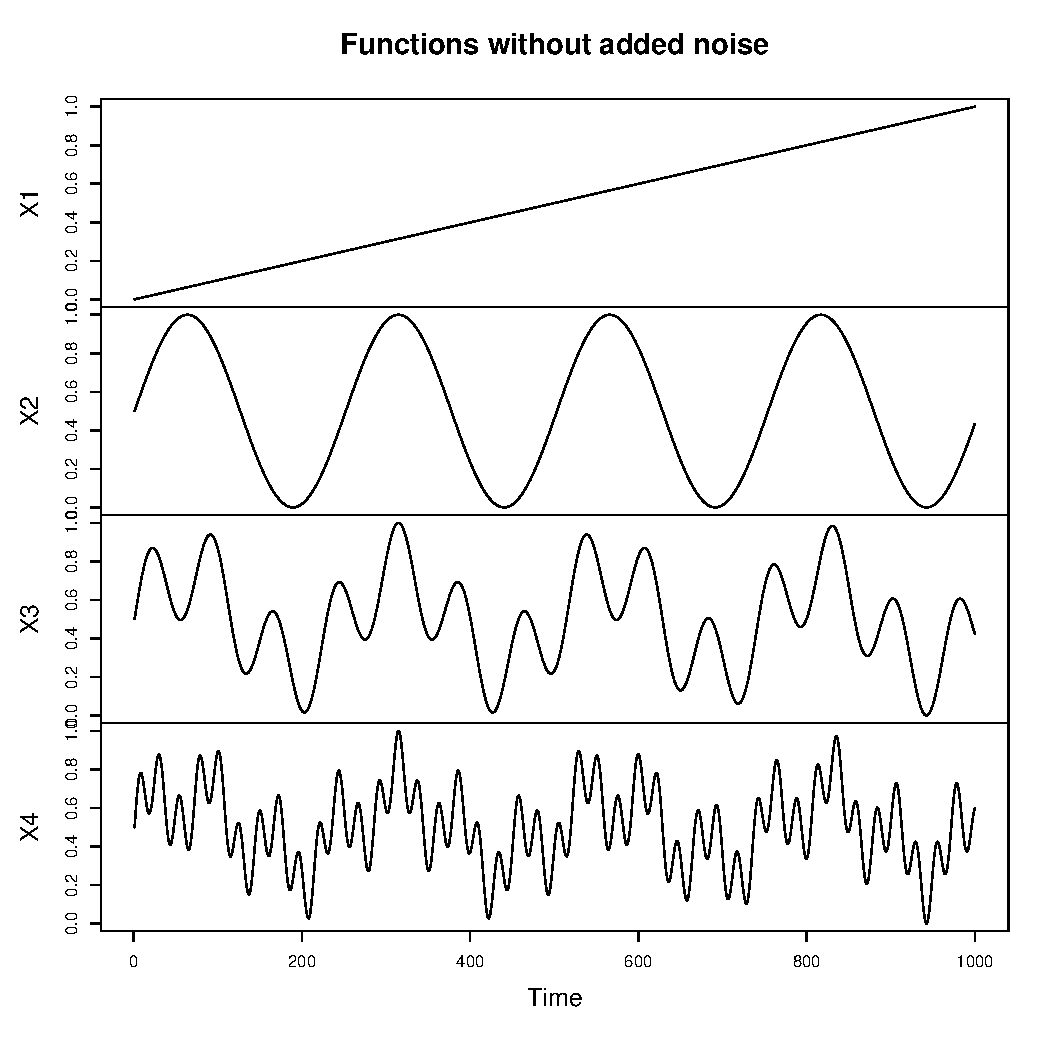
\includegraphics[width = 0.9\linewidth, height = 3in]{./figs/coeff-interp-simple-functions0.pdf}
    % \caption{Functions without added noise.}
    % \label{fig:simple-functions1}
  \end{subfigure}
  \hfill
  \begin{subfigure}[b]{0.45\textwidth}
  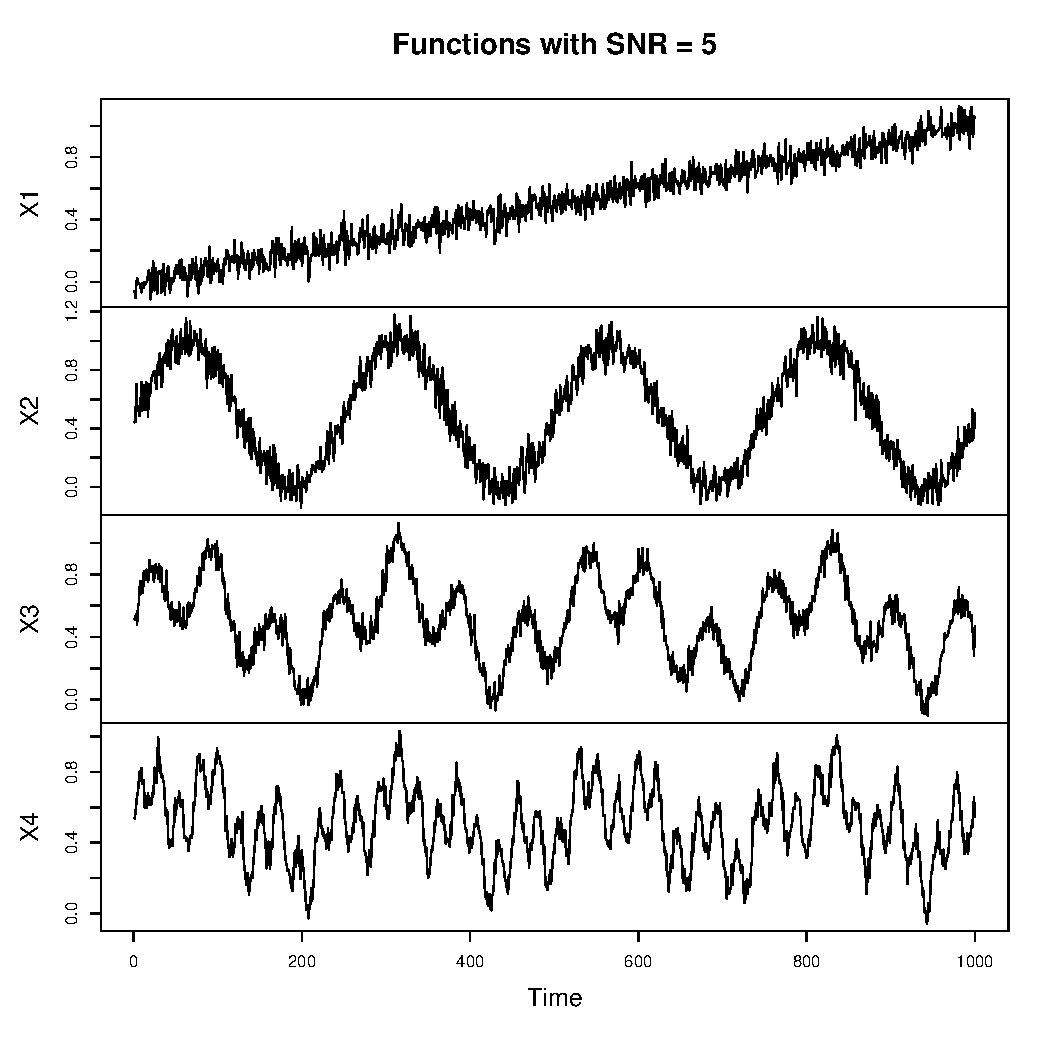
\includegraphics[width = 0.9\linewidth, height = 3in]{./figs/coeff-interp-simple-functions1.pdf}
  % 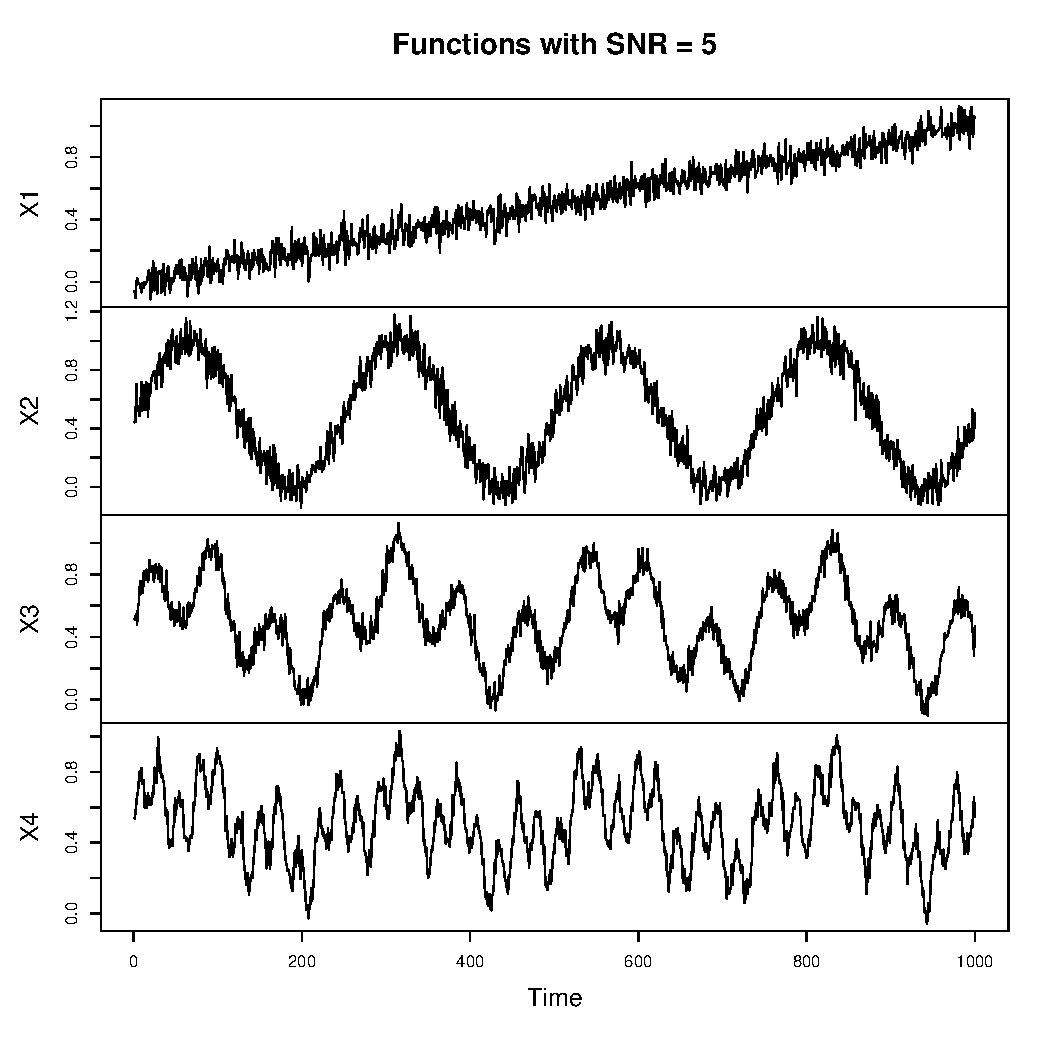
\includegraphics[width = 0.9\linewidth, height = 3in]{./figs/coeff-interp-simple-functions1.pdf}
    % \caption{Functions without added noise.}
  \end{subfigure}
  \caption{Linear and sinusoidal functions with and 
  without added noise.}
     \label{fig:simple-functions}
\end{figure}

  \begin{figure}[h]
    \begin{center}
    % \begin{picture}(60,60)
    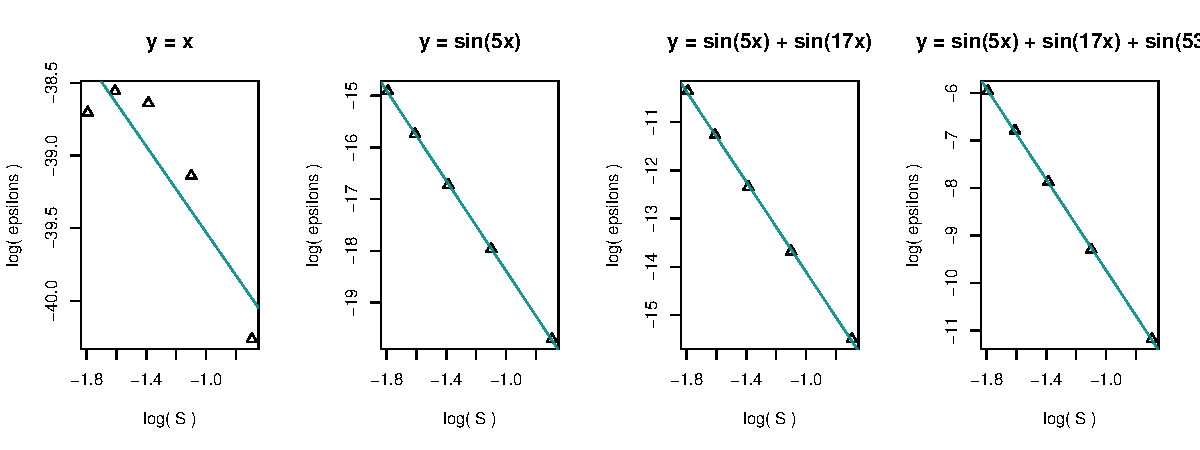
\includegraphics[width = \textwidth, keepaspectratio]
    {./figs/coeff-interp-simple-fits.pdf}
    % \end{picture}s 
    \end{center}
    \caption{The log-log linear regression
     of approximation errors against the
     proportion of sampled $S_h$ for simple 
     linear and sinusoidal functions.}
    \label{fig:simple-fits}
  \end{figure}

% \begin{figure}[!htbp]
%   \begin{center}
%   % \begin{picture}(60,0)
%   \includegraphics[totalheight = 3.4in]
%   {./figs/coeff-interp-simple-functions0.pdf}
%   % \end{picture}
% \end{center}
% \end{figure}
% \begin{figure}[!htbp]
%   \begin{center}
%   % \begin{picture}(60,60)
%   \includegraphics[totalheight = 3.4in]
%   {./figs/coeff-interp-simple-functions1.pdf}
%   % \end{picture}
% \end{center}
% \end{figure}

% (fig: simple-functions)

The epsilon complexity coefficients $A$ and $B$ along with 
a variogram-based fractal dimension estimator which 
we denote $\hat D$, were estimated on the four 
functions depicted in in Figure \ref{fig:simple-functions}. 
In addition to the original functions, $A,B$ and $\hat D$ where 
computed on the functions with two levels of added noise. 
Figure \ref{fig:simple-fits} 
shows the $log-log$ regression of the errors $\varepsilon_h$ 
on the fraction of samples kept $S_h$. The complexity coefficients for these fits are given in Table \ref{tab:simple-coeffs}. While these functions do not reveal much about the behavior of the complexity coefficients for more complicated time series, the results
demonstrate properties of the complexity coefficients and 
the sensitivity of the estimators to added noise.

\begin{table}[!htbp] \centering 
\begin{tabular}{@{\extracolsep{1pt}} ccccccc} 
\\[-1.8ex]\hline 
\hline \\[-1.8ex] 
Without Noise     &  $A$ & $B$  & $\hat D$ \\ \hline 
        $x $    &    -41.45 & -1.92  & 1.00\\ 
 $\sin 5x$  &
                  -22.71 & -4.33 & 1.00 \\ 
 $\sin 5x  + \sin 17x$ &
                  -18.71 & -4.61 & 1.00 \\ 
 $\sin 5x  + \sin 17x + \sin 53x $ &
                  -14.54 & -4.81 & 1.01 
 \\ \hline  
% \hline \\[-1.8ex] 
                 % \end{tabular} 
% \begin{table}[h]
% \begin{center}
%   \begin{tabular}{ | c | c |  c| c| } 
%    
SNR = 20  & $A$ & $B$ & $\hat D$ \\  \hline
$x  $ &
   -4.04  & -0.57   &  1.97 \\  
 $\sin 5x   $ &  
   -3.90  & -0.59   &  1.94 \\  
 $\sin 5x  + \sin 17x  $ &
   -4.07  & -0.55   &  1.94 \\  
$\sin 5x  + \sin 17x + \sin 53x $ & 
   -4.12  & -0.52   &  1.67 
\\ \hline 
SNR = 5    & $A$ & $B$& $\hat D$  \\ \hline
$ x$ &
 -3.39 & -0.54   &  1.99  \\ 
 $\sin 5x $ &
 -3.48 & -0.55   &  1.99  \\ 
 $\sin 5x  + \sin 17x $ &
 -3.58 & -0.55   &  1.99  \\ 
 $\sin 5x  + \sin 17x + \sin 53x $ &
 -3.70 & -0.58   &  1.82  \\
 \hline \\[-1.8ex] 
    \end{tabular}
  \caption{Complexity coefficients and fractal dimension
  estimates for linear and sinusoidal functions.}\label{tab:simple-coeffs}  
\end{table}

The parameters of the linear regression in Figure 
\ref{fig:simple-fits} determine the complexity 
coefficients $A,B$. The $x-$axis is the log of $S_h$, 
the proportion of points used to approximate the original function at each step. The finest scale approximation is when $h=2$, represented by the point with the least (log) error located furthest to the right at $log( S )\approx -0.7$. Small values at this point
 correspond to accurate approximations and less variability at the finest scale of the sampled function. 
In theory, the approximation error at zero should be an exact approximation of the function. Since we are computing the log of the approximation error $\varepsilon$, $\log(\varepsilon) \to -\infty$
as $\varepsilon \to 0$. For 
the three functions in Figure \ref{fig:simple-functions}
the overall approximation error is low. Larger intercept 
should correspond to larger errors and, as expected, 
the intercept value $A$ increases with increased
function complexity and higher levels of noise.  

The complexity coefficient $B$ measures the rate of change 
of the approximation error as a function is approximated
using fewer samples. The coefficient $B$ increases rapidly 
as noise is added. Similarly, the fractal dimension estimator
approaches its theoretical maximum 2  
as Gaussian noise is added to the functions.
In order to compare these results to estimates on 
pure Gaussian noise, we estimated the complexity coefficients
and fractal dimension on 50 samples Gaussian noise. The 
mean estimate of the complexity coefficient $B$ was $-0.54$, 
close to the estimates in Table \ref{tab:simple-coeffs} for 
functions with added noise. For both the fractal dimension 
estimator and the complexity coefficient $B$, relatively 
small amounts of added noise generate estimates similar to 
that of Gaussian noise.

\begin{table}[!htbp] \centering 
\begin{tabular}{@{\extracolsep{1pt}} ccccccc} 
\\[-1.8ex]\hline 
\hline \\[-1.8ex] 
              &  $A$  & $B$  & $\hat D$ \\ \hline
 White Noise  & -2.84 & -0.54 & 2 \\ \hline
    \end{tabular}
  \caption{Complexity coefficients and fractal dimension estimates
   for Gaussian noise.}
  \label{tab:white-noise}  
\end{table}

\section{H\"older Class and Fractal Dimension}

% Theorem \ref{thm:holder} states a relationship 
% between a H\"older class of functions 
% and the complexity coefficients. The proof of the theorem differs in some details from the method of estimating the complexity coefficients. 
% For example, the proof assumes the error is 
% achieved by taking the infimum over a possibly 
% infinite family of functions $\mathcal{F}$,  
% and the max norm rather than the Euclidean 
% norm. In addition, the statement relates
% the $\varepsilon-$complexity to a class 
% H\"older continuous functions, although the 
% same relation should hold for individual members
% of that H\"older class.


Several of the simulations used in Chapter 3 to test the 
performance of approximation methods have  parameters that 
determine both the H\"older class of a function and its 
fractal dimension. Our experiments show that for most 
of these simulations, the complexity slope coefficient 
$B$ behaves similar to the variogram estimator of
fractal dimension $\hat D$. For three of the simulations, 
the Weierstrass function, fractional Brownian motion(fBm), 
and the Cauchy process, the median values of the 
$B$ and $\hat D$ change linearly with the parameters 
determining both fractal dimension and the H\"older 
exponent of the function or sample paths of the simulations.
For these simulations, the complexity intercept coefficient $A$
changed non-linearly as the parameter determining the 
H\"older class of a function changed. A different 
pattern was observed for the random-phase
Weierstrass function. For samples of the random- 
phase Weierstrass function, the values for the 
complexity coefficient $B$ and $\hat D$ were similar 
to white noise while the complexity
coefficient $A$ changed linearly with the parameter 
deterimining the H\"older exponent of the function.


The Weierstrass function is a self-similar 
deterministic function 
whose H\"older exponent and fractal dimension when 
written
\begin{align}
      W_{\alpha}(x) 
  \hspace{1em}= \sum_{n = 0}^{\infty} b^{-n \alpha} \cos(b^n \pi x)
\end{align}
is determined by the single parameter $\alpha$. The 
H\"older exponent is equal to $\alpha$ while the functions
fractal dimension is $D = 2 - \alpha$. 
Since the function is deterministic, the complexity 
coefficients and fractal estimator were calculated 
on a single example of length 1000 for 20 parameters 
of $\alpha$ in the interval $(0,1)$. The results 
in Figure \ref{fig:notrandom-params}  
show that the complexity coefficient $B$ and fractal dimension
change linearly with $\alpha$. The fractal dimension 
estimator tracks the theoretical fractal dimension 
closely, ranging from 2 to 1. The complexity coefficient 
$B$ ranges $-0.6$ to $-1.4$. For both estimators, fractal 
dimension corresponding to 2 coincides with estimates
close to those estimated for Gaussian noise.

The random-phase Weierstrass function adds a random 
phase to the periodic component of the Weierstrass function 
but its H\"older exponent and fractal dimension are 
determined by the $\alpha$ parameter
in the same manner as for the deterministic 
Weierstrass function.The Weierstrass and 
random-phase Weierstrass functions are
 illustrated in Figure \ref{fig:weierstrass} 
for three different parameter values $
\alpha = \{ 0.20, 0.42, 0.80 \}$. Unlike the other 
results reported in this Chapter, neither the 
fractal estimator nor the complexity coefficient 
$B$ varied with $\alpha$. For each parameter the complexity coefficients 
and fractal dimension were estimated on 50 
samples of length 1000. Figure 
\ref{fig:rp-weierstrass-boxplot} shows that the 
complexity coefficient $B$ and
fractal estimator $\hat D$ range around values 
associated with estimates for Gaussian noise.
The intercept coefficient $A$ increases 
linearly but the total magnitude of the change is 
relatively small--- the median of the estimates has a range 
of less than $0.5$. 


\begin{figure}[h]
  \begin{subfigure}[b]{0.49\textwidth}
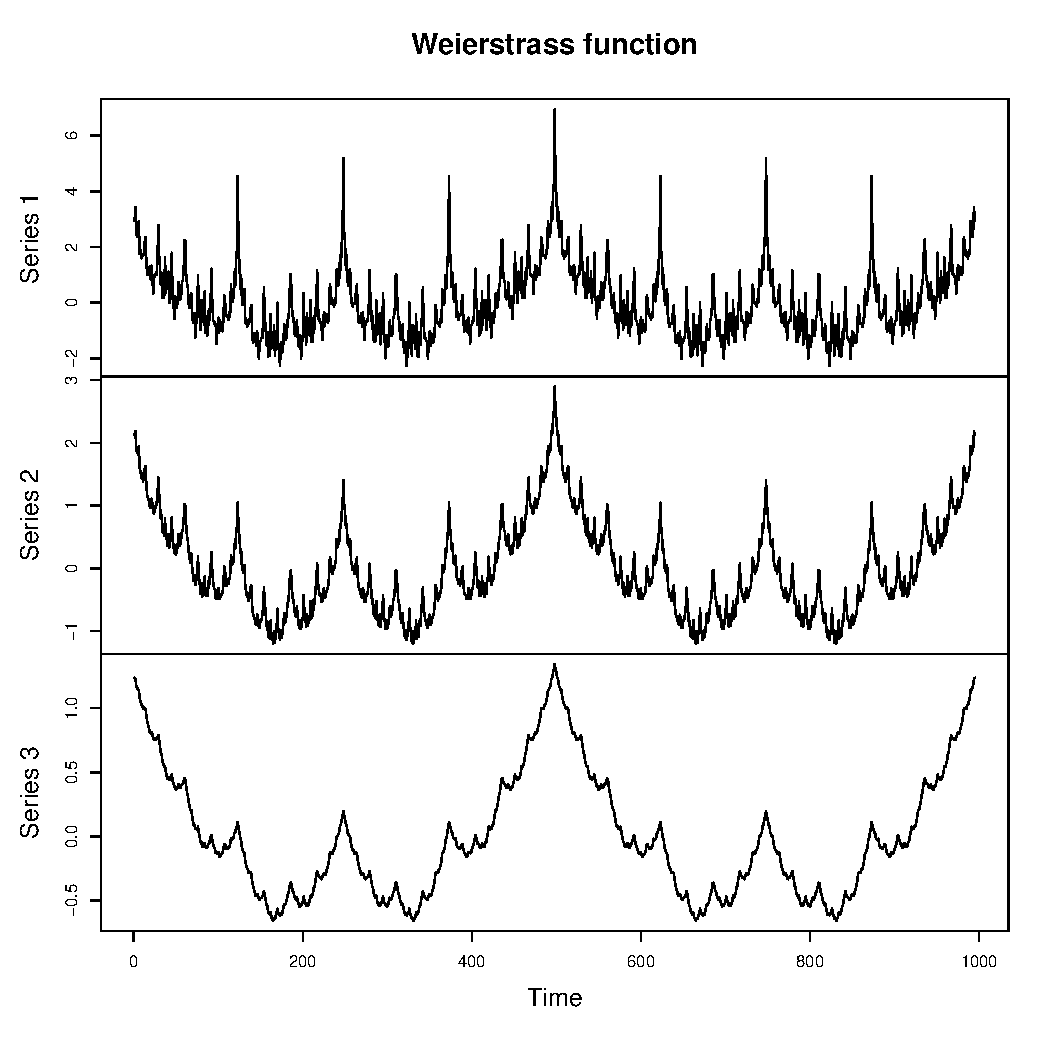
\includegraphics[width = 0.9\linewidth, height = 3in]{./figs/holder_notrandom-weier-notrandom.pdf}
    % \caption{Functions without added noise.}
    \label{fig:weierstrass}
  \end{subfigure}
  \hfill
  \begin{subfigure}[b]{0.49\textwidth}
  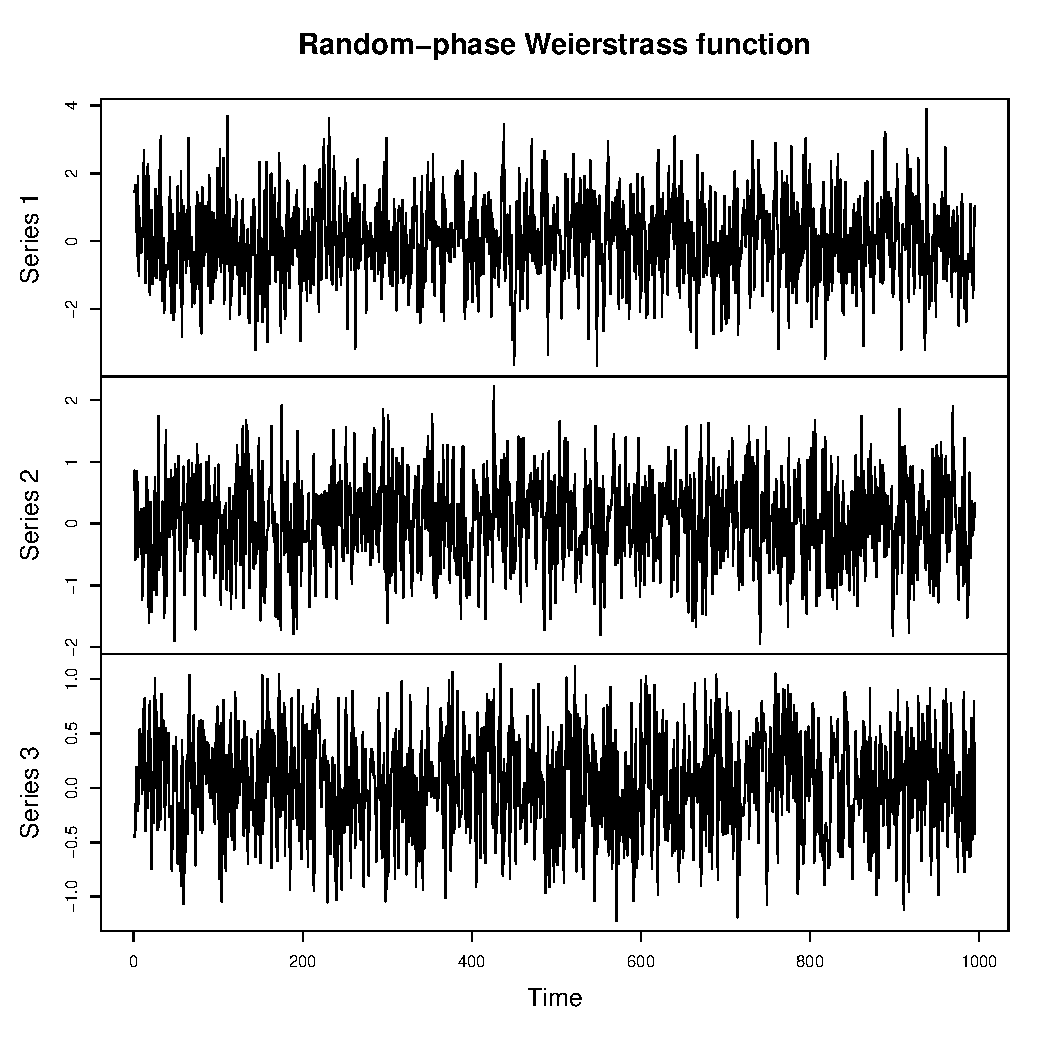
\includegraphics[width = 0.9\linewidth, height = 3in]{./figs/holder_coeffs-weier-random.pdf}
    % \caption{Functions without added noise.}
  \end{subfigure}
  \caption{The Weierstrass and random-phase Weierstrass function
  for $\alpha = \{ 0.20, 0.42, 0.80 \}$}
    \label{fig:weierstrass}
\end{figure}

\begin{figure}[!htbp]
  \begin{center}
  % \begin{picture}(60,60)
  % ./figs/coeff-interp-simple-functions1.pdf
  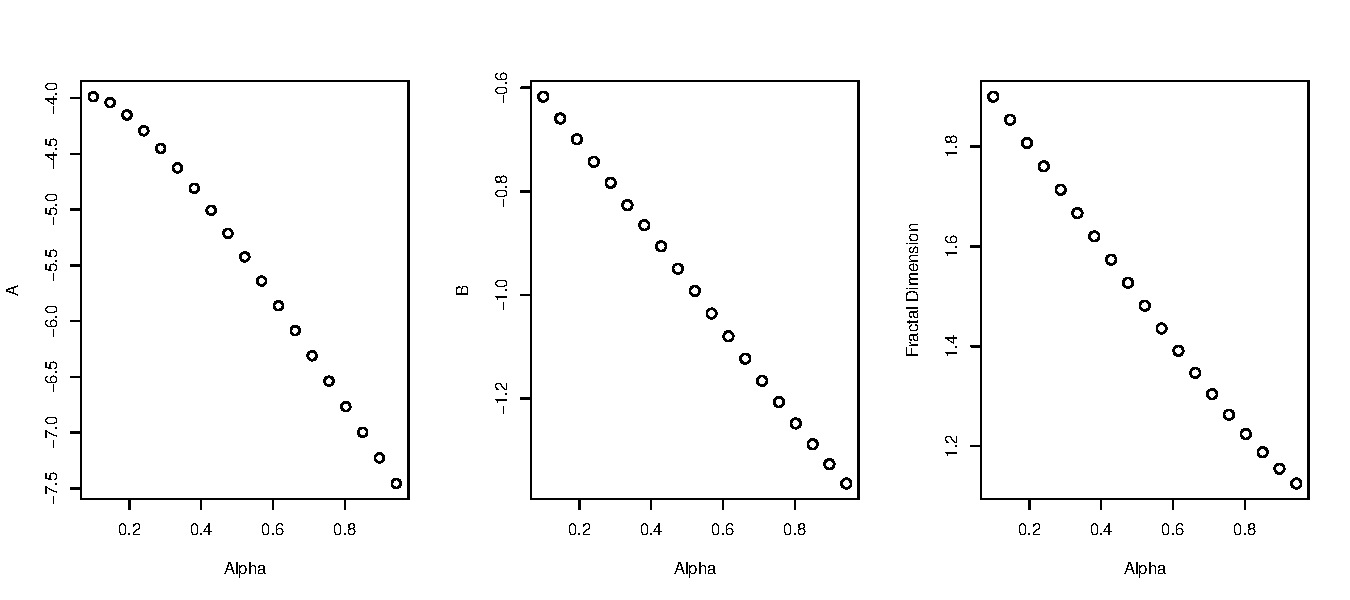
\includegraphics[width = \textwidth, keepaspectratio]{./figs/holder_notrandom-param-plots-notrandom.pdf}
  % \end{picture}
  \end{center} 
  \caption{Complexity coefficients and fractal dimension 
    for values of the Weierstrass $\alpha$ parameter.  }
  \label{fig:notrandom-params}
\end{figure}


Fractional Brownian motion also has 
a single parameter $\alpha$ which is equal to
 the H\"older exponent and determines the fractal dimension of
sample paths as $D = 2 - \alpha$. For fBM the 
parameter $\alpha$, sometimes denoted $H$, is also 
the Hurst parameter. The results 
of the estimators computed on 50 samples are shown 
in Figure \ref{fig:fbm-boxplots} and are similar 
to the estimates for the deterministic Weierstrass 
function with the median of both the complexity
coefficient $B$ and $\hat D$ changing linearly
with the parameter $\alpha$. As was
the case for the deterministic Weierstrass 
function, the complexity 
coefficient $A$ also changes non-linearly with 
$\alpha$.

% Figure \ref{fig:notrandom-B-fd}
% shows that the complexity coefficient $B$ changes 
% linearly with the fractal estimator $\hat D$. 


% The simulati
% do not have an explanation for the discrepancy between 
% the theoretical H\"older class and fractal dimension 
% of the function and the results of the simulation. Unlike the determinstic Weierstrass 
% function and the Cauchy and Fractional Brownian 
% motion processes, the graph of the random-phase 
% Weierstrass did not become locally smoother as 
% $\alpha$ was increased and the coefficient $B$ and 
% estimator $\hat D$ are numerically similar to the results 
% given when white noise was added to the simple functions 
% as reported in Table \ref{tab:simple-coeffs}.

\begin{figure}[!htbp]
  \begin{center}
  % \begin{picture}(60,60)
  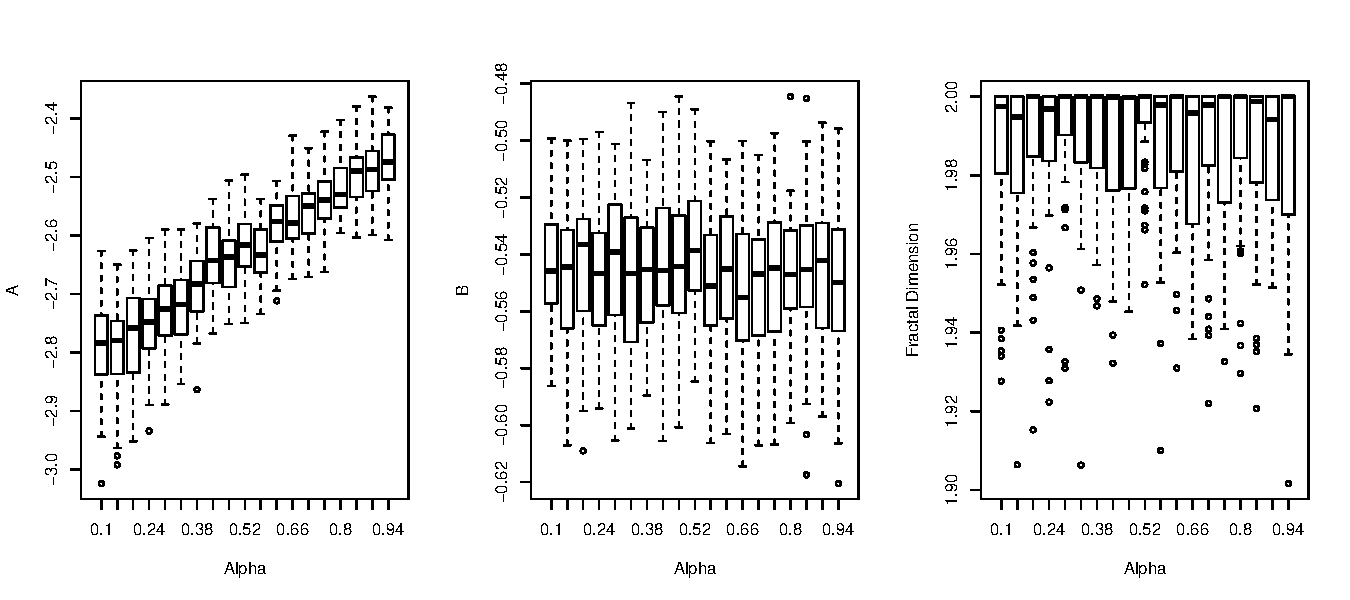
\includegraphics[height = 3in, width =6in, keepaspectratio]{./figs/holder_coeffs-boxplots.pdf}
   
  \caption{Complexity coefficients and fractal dimension 
   for values of the random-phase
    Weierstrass $\alpha$ parameters.  }
  % \end{picture}
    \label{fig:rp-weierstrass-boxplot}
  \end{center}
\end{figure}


\begin{figure}[!htbp]
  \begin{subfigure}[b]{0.49\textwidth}
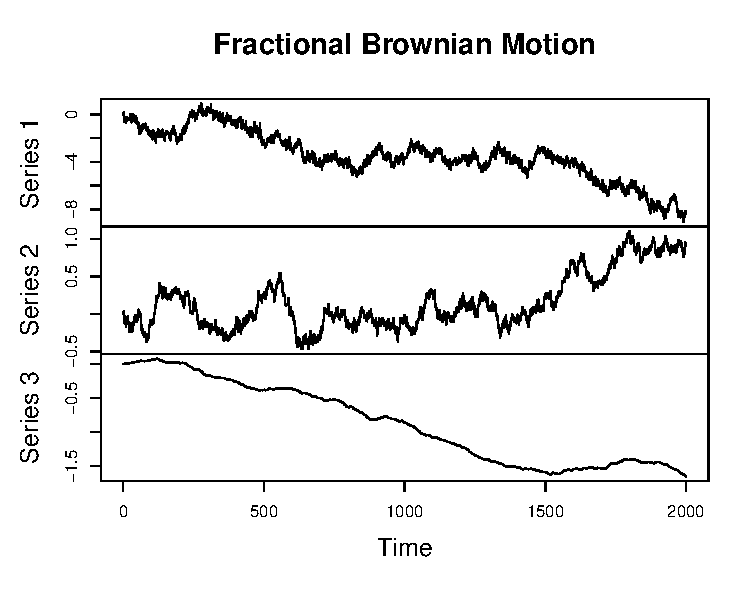
\includegraphics[width = 0.9\linewidth, height = 3in]{./figs/fBm-coeffs-plot.pdf}
    % \caption{Functions without added noise.}
    % \label{fig:fBmplot}
  \end{subfigure}
  \hfill
  \begin{subfigure}[b]{0.49\textwidth}
  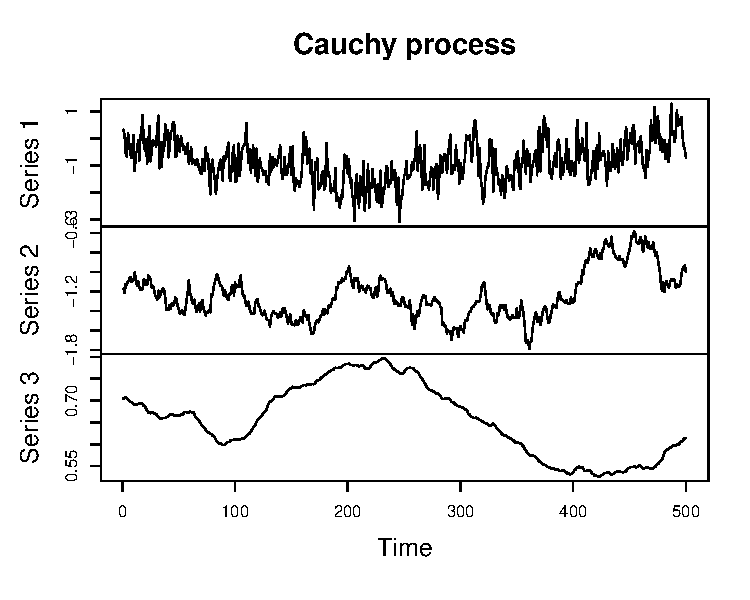
\includegraphics[width = 0.9\linewidth, height = 3in]{./figs/cauchy-plot.pdf}
    % \caption{Functions without added noise.}
    
  \end{subfigure}
  
  \caption{Fractional Brownian motion and the Cauchy process with $\alpha = \{ 0.20, 0.42, 0.80 \}$ for a constant $\beta$ parameter.}
\end{figure}

\begin{figure}[!htbp]
  \begin{center}
  % \begin{picture}(60,60)
  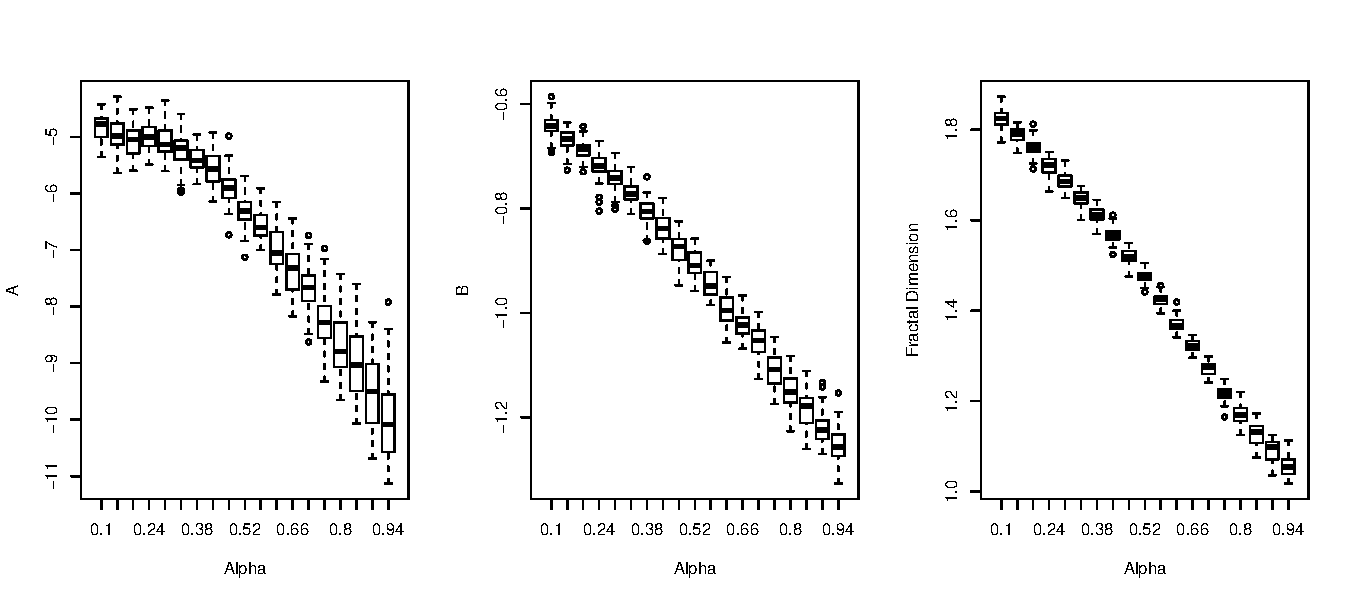
\includegraphics[height = 3in, width =6in, keepaspectratio]{./figs/fBm-coeffs-boxplots.pdf}
  % \end{picture}
  \end{center}
  \caption{Complexity coefficients and fractal dimension for 
  values of the $\alpha$ parameter of fractional Brownian motion.} 
    \label{fig:fbm-boxplots}
\end{figure}

\begin{figure}[!htbp]
  \begin{center}
  % \begin{picture}(60,60)
  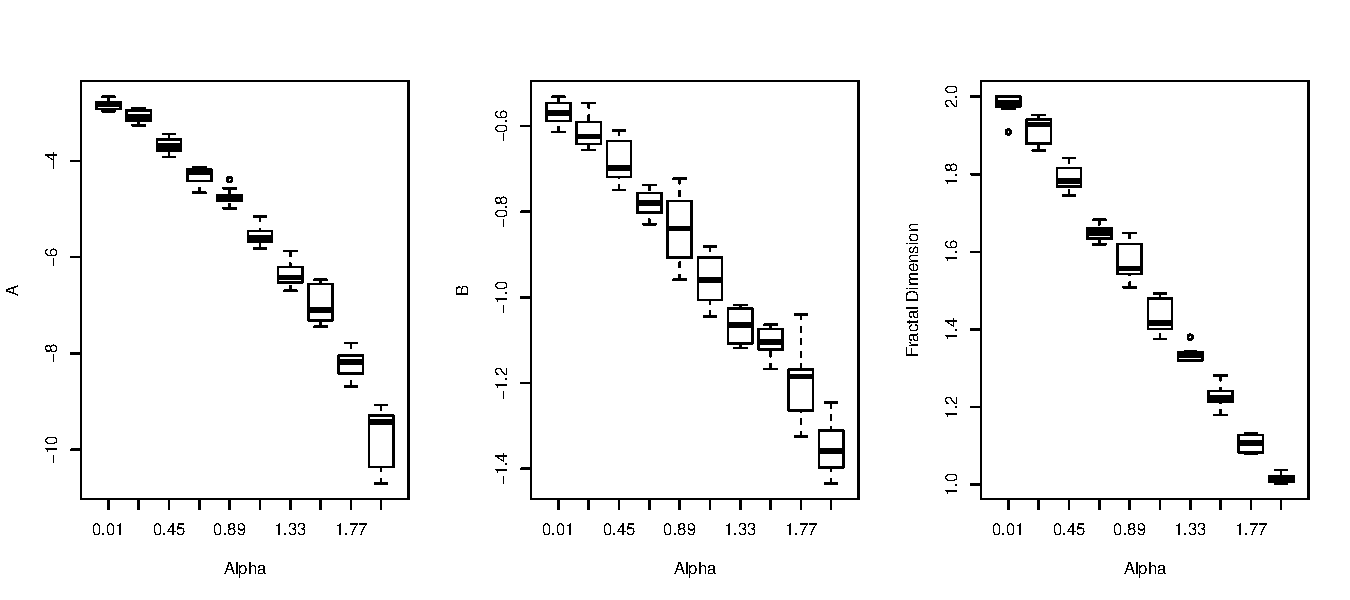
\includegraphics[height = 3in, width =6in, keepaspectratio]{./figs/cauchy-boxplots.pdf}
  % \end{picture}
  \end{center}
  \caption{Complexity coefficients and fractal dimension for 
  various $\alpha$ parameters for a constant $\beta$ parameter
  of the Cauchy process.} 
     \label{fig:cauchy-boxplots}
\end{figure}


The Cauchy process was the final simulation we tested.
The Cauchy process has two parameters: the 
parameter $\alpha$ determines
fractal dimension and the parameter $\beta$ determines 
the Hurst coefficient or long-range dependence of 
the sample paths. Simulations were generated on a 
grid of the parameters $\alpha, \beta$ 
for $0 < \alpha < 2$ and $0 < \beta < 1.5$ with 30 simulations
generated for each point on the parameter grid. At a 
constant parameter $\beta$ the median of the complexity 
coefficients and fractal estimator again show a linear
relation to the $\alpha$ parameter, as shown 
in Figure \ref{fig:cauchy-boxplots}. This relation holds 
even as $\beta$, the Hurst parameter, is varied. The 
mean value of each of the estimators for for a fixed 
value $\beta$ and $\alpha$ is shown in Figure 
\ref{fig:cauchy-alpha}. Variation in the Hurst parameter
has little affect on the either the complexity coefficients
or the fractal dimension estimator.


\begin{figure}[!htbp]
  \begin{center}
  % \begin{picture}(60,60)
  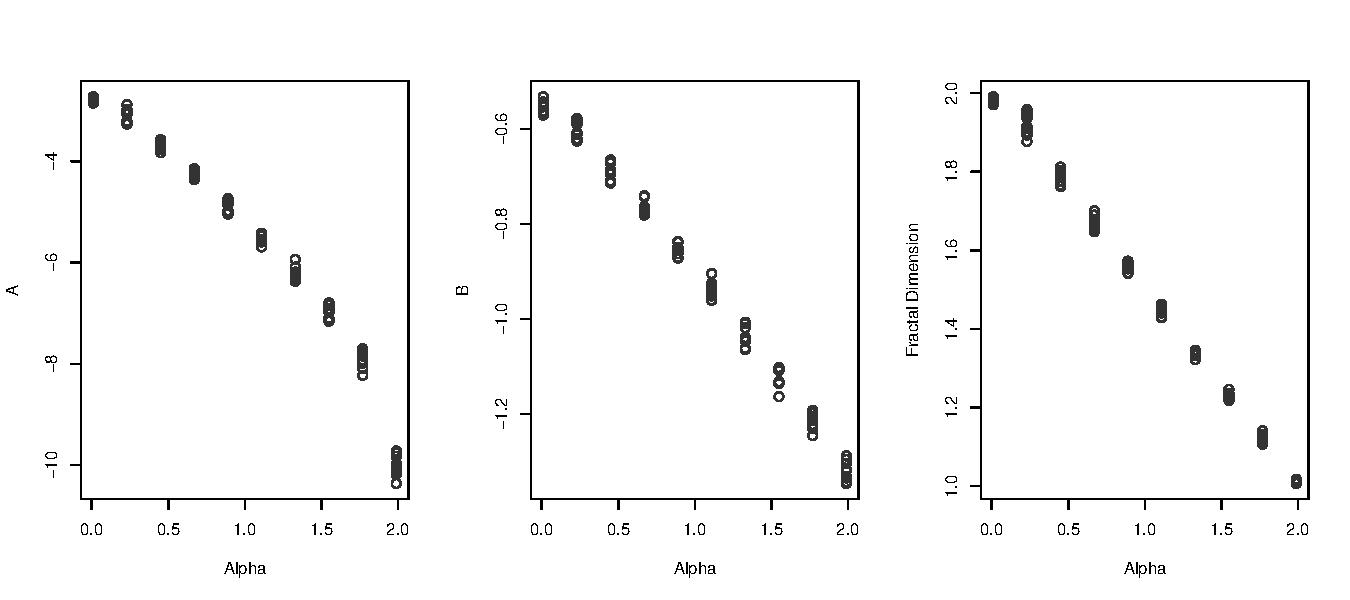
\includegraphics[height = 3in, width =6in, keepaspectratio]{./figs/cauchyalpha-scatterplots.pdf}
  % \end{picture}
  \end{center}
  \caption{Mean value of the complexity coefficients and fractal dimension for each $\alpha$ value of the Cauchy process.}
   \label{fig:cauchy-alpha}
\end{figure}

\begin{figure}[h]
  \begin{center}
  % \begin{picture}(60,60)
  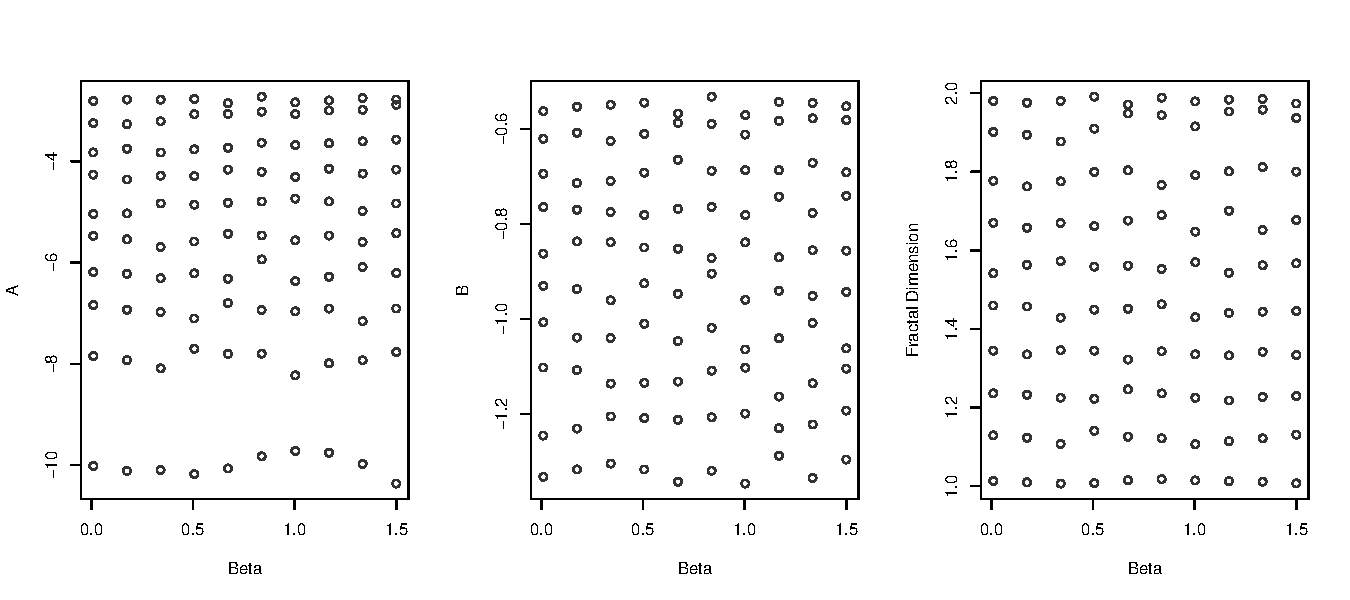
\includegraphics[height = 3in, width =6in, keepaspectratio]{./figs/cauchybeta-scatterplots.pdf}
  % \end{picture}
  \end{center}
  \caption{The mean value of the complexity coefficients and fractal dimension for each $\beta$ value of the Cauchy process.}
 \label{fig:cauchy-beta}
\end{figure}

Figure \ref{fig:cauchy-beta} shows another view of 
the complexity coefficients plotted against 
changes the Cauchy process parameter $\beta$. The complexity 
coefficient $B$ and fractal dimension $\hat D$, 
 preserve the grid of the parameter space --- for a fixed 
$\beta$, the parameter varies linearly with $\alpha$. The  
$\beta$ parameter controls the long-range dependence of 
the Cauchy process and the plots indicate that 
the complexity coefficients, like fractal dimension,
measure a local, property of a function.


For all simulations but the random-phase Weierstrass function 
the, a similar pattern was observed for the complexity 
coefficients and the fractal dimension estimator. Both 
the fractal dimension estimator $\hat D$ and the complexity 
coefficient $B$ changed linearly with the parameter
determining the H\"older exponent and fractal dimension of 
the simulations. 
 On the other hand, our initial example of simple functions and the random-phase Weierstrass functions appears shows a relationship between the intercept 
coefficient $A$ and fine-scale noise. These results are for a small set of processes whose fractal dimension and H\"older exponent are
determined by a single paramater. A comparison of the complexity coefficient $B$ and fractal estimators on a wider variety of time series might show whether the relation the $\varepsilon$-complexity coefficients and fractal dimension hold for a wider range 
conditions. 

% The variogram estimator of fractal dimension takes the log-log relation of $h$ to $E(x(t+h) x(t))^2$ over a range of increments $h$. On the other hand, the complexity coefficients compute the approximation using only samples taken at intervals $h$ over range of increments.  























